%%=============================================================================
%% Proof of concept
%%=============================================================================
\chapter{Proof of concept}
\label{ch:proof-of-concept}
%TODO cpations bij figuren nakijken

%Wat wil je bewijzen of aantonen met deze PoC?
De hoofddoelstelling van deze PoC is te onderzoeken hoe een LLM ondersteuning kan bieden binnen een IT-supportsysteem, met als doel technische IT-vragen sneller af te handelen. De toepassing is bedoeld voor intern gebruik door het MyMinfin IT-team en niet voor externe gebruikers, zoals burgers. In de stand van zaken werden verschillende benaderingen onderzocht. In dit hoofdstuk wordt een keuze gemaakt uit deze benaderingen en toegepast op de PoC.
\\[1em]
%Welke hypothese test je eigenlijk?
De hypothese die binnen deze PoC getest wordt, kan als volgt worden samengevat:
\textit{“Kan een LLM effectief en efficiënt ondersteuning bieden binnen een IT-supportsysteem door relevante informatie uit documentatie te halen en daarmee het supportproces te optimaliseren en te vereenvoudigen.”}

\section{Behoeften analyse}
Voor de PoC werd een interview afgelegd. Op basis van dit interview werd een MoSCoW-analyse uitgevoerd om de functionele vereisten te prioritiseren. De analyse werd onderverdeeld in \textit{Must haves}, \textit{Should haves} en \textit{Could haves}

\subsection{Must haves}
\begin{itemize}
    \item \textbf{Vragen kunnen stellen in de eigen taal (bijvoorbeeld Nederlands, Frans of Engels)}:\\ 
    Het systeem moet correct functioneren ongeacht of de gebruiker vragen stelt in het Nederlands, Frans of Engels.
    \item \textbf{Een duidelijk en bruikbaar antwoord ontvangen op basis van betrouwbare bronnen}:\\ 
    De gegenereerde antwoorden moeten informatief, relevant en praktisch toepasbaar zijn.
    \item \textbf{Eenvoudige en intuïtieve interface}:\\  
    De gebruiker mag geen technische kennis nodig hebben. De interactie moet vanzelfsprekend en gebruiksvriendelijk aanvoelen.
    \item \textbf{Consistente ervaring (snel, zonder fouten of willekeurige antwoorden)}:\\  
    De gebruiker verwacht dat de applicatie betrouwbaar functioneert en consistente resultaten levert.
\end{itemize}

\subsection{Should haves}
\begin{itemize}
    \item \textbf{Het systeem begrijpt vervolgvragen binnen een sessie}:\\  
    De gebruiker moet een gesprek kunnen voeren waarbij eerdere vragen worden meegenomen in de context, zodat interacties natuurlijker verlopen.
    \item \textbf{Transparantie over de gebruikte bronnen van het antwoord}:\\  
    De gebruiker moet kunnen zien uit welk document of welke bron het antwoord afkomstig is, zodat de informatie steeds gecontroleerd en gevalideerd kan worden.
\end{itemize}

\subsection{Could haves}
\begin{itemize}
    \item \textbf{Langetermijngeheugen over meerdere sessies heen}:\\  
    Het opzetten van een geheugen dat sessie-overstijgend werkt, brengt extra complexiteit met zich mee en is daarom minder geschikt voor een eerste versie.
    \item \textbf{Zelf documenten kunnen uploaden of bewerken}:\\  
    In deze PoC ligt de focus op het zoeken en beantwoorden van vragen, niet op het beheren van documenten.
    \item \textbf{Automatisch mails behandelen}:\\  
    Het automatisch verwerken en beantwoorden van e-mails valt qua complexiteit buiten de scope van een eerste versie.
\end{itemize}

\section{Architectuur en Ontwerp}

Vooraleer de structuur van de PoC kan worden opgezet, moet een keuze gemaakt worden voor de meest geschikte techniek. Fine-tuning is, gelet op de scope van de PoC, moeilijk uitvoerbaar. Om dit te realiseren zou een model getraind moeten worden op data die kan helpen bij IT-support. Hoewel er data beschikbaar is in de vorm van e-mails, is het onderhoud bij fine-tuning niet te onderschatten. Wanneer een procedure of bepaalde gegevens veranderen, moet het model immers opnieuw getraind worden. Deze keuze brengt met andere woorden een hoge initiële kost met zich mee en potentieel ook een hoge onderhoudskost, die niet aanwezig is bij RAG of CAG.
\\[1em]
Met CAG aan de andere kant zouden alle documenten worden toegevoegd aan de context. Hoewel dit technisch mogelijk is, zeker met de modellen van vandaag, heeft deze aanpak enkele nadelen. Ten eerste kan \textit{context rot} een probleem vormen. Zoals aangegeven in de stand van zaken, worden modellen minder performant wanneer te veel informatie in de context wordt geplaatst. Daarnaast wordt bij CAG niet alleen relevante, maar ook irrelevante informatie toegevoegd. Dit verhoogt niet alleen de kans op minder nauwkeurige antwoorden, maar ook de mogelijke API-kosten in vergelijking met RAG.
\\[1em]
Met al deze redenen in gedachten is voor deze PoC gekozen om RAG toe te passen. Enerzijds zijn er geen hoge initiële kosten zoals bij fine-tuning, en anderzijds worden enkel relevante documenten toegevoegd aan de context. Dit helpt om mogelijke problemen van context rot te vermijden en houdt bovendien de kost per query laag. Tabel \ref{tab:techniek_vergelijking} geeft een overzicht van de voor- en nadelen van de verschillende benaderingen.

\begin{table}[H]
    \resizebox{\textwidth}{!}{
            \begin{tabular}{|p{4cm}|c|c|c|}
            \hline
            \textbf{Kenmerk} & \textbf{Fine-tuning} & \textbf{CAG} & \textbf{RAG} \\
            \hline
            Initiële kost & Hoog & Laag & Laag \\
            \hline
            Onderhoudskost & Hoog & Laag & Laag \\
            \hline
            Document selectie & n.v.t -- kennis zit in model & Alle documenten & Enkel relevante \\
            \hline
            Kost per query & Laag & Potentieel hoog  & Laag \\
            \hline
            Implementatie & Complex door training model & Relatief eenvoudig & Complex door implementatie retrieval\\
            \hline
        \end{tabular}
    }
    \caption{Vergelijking van voor- en nadelen van fine-tuning, CAG en RAG}
    \label{tab:techniek_vergelijking}
\end{table}

\subsection{Algemene structuur}

Deze structuur bestaat uit een graaf die is opgebouwd uit verschillende knooppunten (nodes). De graaf stelt de LLM in staat om zelfstandig te bepalen welke keuzes gemaakt moeten worden tijdens het verwerken van een vraag.
\\[1em]
De standaard RAG-architectuur gaat een query gaan embedden en haalt vervolgens de meest relevante documenten op uit de vectordatabase, zonder verdere reflectie over de nood van het ophalen van de documenten en de werkelijke relevantie van deze documenten. Hoewel dit op het eerste gezicht een efficiënte aanpak lijkt, betekent het ook dat het systeem bij elke willekeurige gebruikersvraag opnieuw de vectordatabase bevraagt, zelfs wanneer dat niet noodzakelijk is.
\\[1em]
Om dit te vermijden, werd gebruikgemaakt van een graafstructuur die het model de mogelijkheid geeft om zelf te beoordelen wanneer het relevant is om documenten op te halen. Daarnaast wordt de LLM ook verantwoordelijk geacht om te oordelen over de opgehaalde documenten. De volledige flow van het proces kan worden bekeken in figuur~\ref{fig:Architectuur}
\\[1em]
De PoC werd uitgewerkt met behulp van Ollama, een tool waarmee open modellen op lokale hardware kunnen functioneren. Tijdens overleg met de betrokken partijen werd geen voorkeur uitgesproken voor specifieke modellen, enkel het gebruik van DeepSeek modellen werd afgeraden.

\begin{figure}[H]
    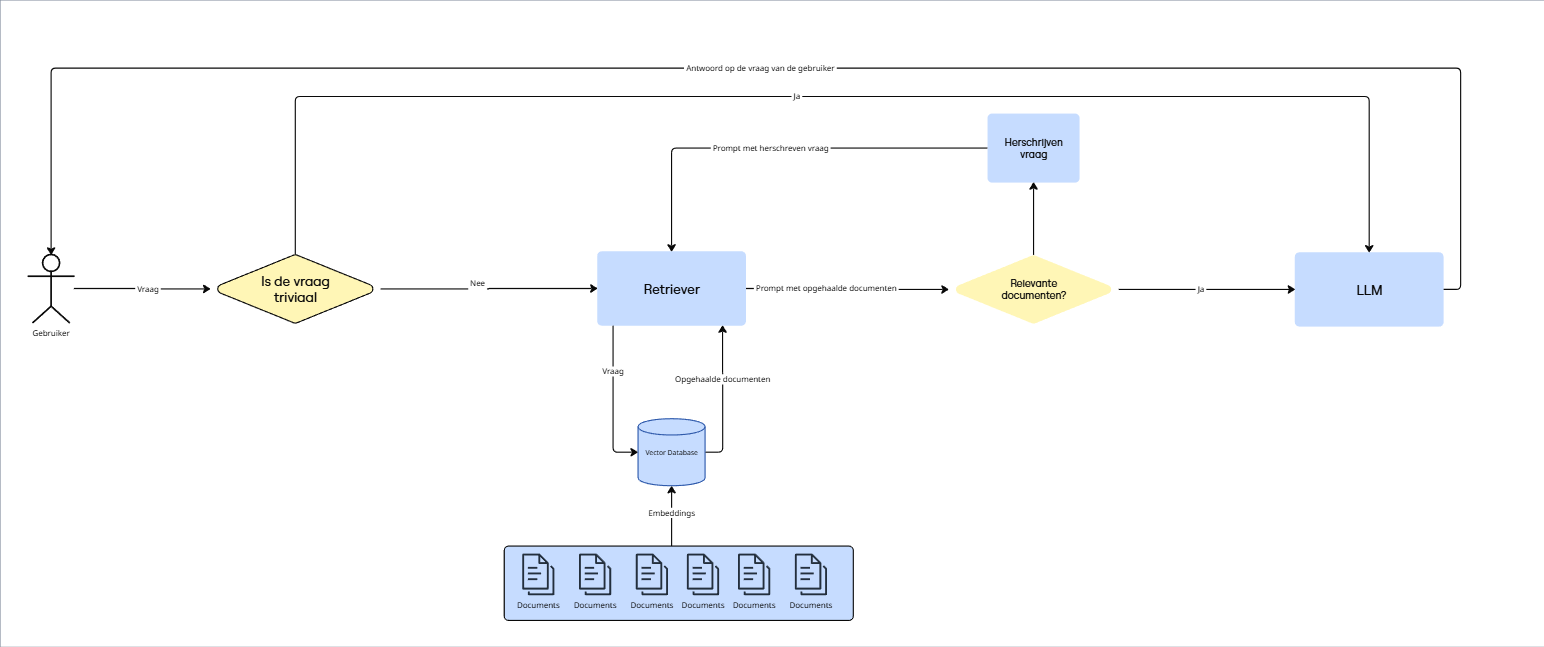
\includegraphics[width=1\textwidth]{flowchart.png}
    \caption{Architectuur van de PoC gebaseerd op een graafgebaseerde workflow. De LLM beslist binnen deze flow of de vectordatabase geraadpleegd moet worden. Bij een database-query beoordeelt de LLM vervolgens of de opgehaalde documenten relevant zijn voor de gestelde vraag. Indien de documenten niet relevant zijn, herschrijft de LLM de vraag en voert de herschreven query opnieuw uit.}
    \label{fig:Architectuur}
\end{figure}

%Belangrijke keuzes tijdens het bouwen (waarom bv. technologie X en niet Y?).

Eén van de belangrijkste beslissingen in deze PoC was de initiële keuze voor RAG ten opzichte van andere mogelijke benaderingen. Eens deze keuze gemaakt was, volgde de selectie van een geschikt framework om RAG te implementeren.
\\[1em]
Voor deze PoC werd gekozen voor LangGraph, een framework waarmee zogenaamde agents kunnen worden opgebouwd aan de hand van grafen. Dit verschilt van bijvoorbeeld LangChain, waar gewerkt wordt met ketens van opeenvolgende stappen.
\\[1em]
LangGraph biedt meer flexibiliteit om een eigen flow te implementeren. Zo kan een LLM bijvoorbeeld zelf kiezen welke paden in de graaf doorlopen worden, of kan er een lus geïntroduceerd worden binnen de graafstructuur. Beide mechanismen werden effectief toegepast in deze PoC.
\\[1em]
%Qwen3 hypoImage vraag zie je rewrite en 2de poging lukt het wel
Dit is bijzonder nuttig in deze use case omdat er voldaan moet worden aan een meertalige omgeving. Het is vooraf namelijk niet zeker in welke taal de gebruiker de toepassing zal gebruiken. Dit kan Frans, Nederlands of Engels zijn. Daarnaast is de documentatie ook in verschillende talen beschikbaar. Sommige documenten zijn voorhanden in het Frans, terwijl andere in het Engels of Nederlands beschikbaar zijn. Met andere woorden kan een vraag in het Nederlands gesteld worden terwijl de documentatie enkel in het Engels beschikbaar is, wat soms tot problemen leidt in het ophalen van de correcte documentatie. Door te werken met een graaf kan de LLM complexere paden volgen die bijvoorbeeld met LangChain niet realiseerbaar zouden zijn geweest.
\\[1em]
Daarnaast maakt deze aanpak het mogelijk om de vaardigheden van de verschillende modellen te testen. Het is immers aan de LLM zelf om op verschillende momenten in het proces keuzes en inschattingen te maken.

\subsection{Gebruikte tools en frameworks}
Tabel \ref{tab:gebruikte_technologieen} geeft een overzicht van de verschillende frameworks, tools en programmeertalen die werden gebruikt om deze PoC op te stellen.

\begin{table}[H]
    \begin{tabular}{|l|l|}
        \hline
        \textbf{Categorie}       & \textbf{Technologieën}               \\ \hline
        Frameworks/Libraries     & LangChain, LangGraph, Streamlit, Ragas \\ \hline
        Tools                   & ChromaDB, Ollama                    \\ \hline
        Programmeertalen        & Python                             \\ \hline
    \end{tabular}
    \caption{Overzicht van de gebruikte technologieën}
    \label{tab:gebruikte_technologieen}
\end{table}

\section{Implementatie}

In deze sectie wordt de concrete opbouw van de PoC toegelicht. Er wordt stap voor stap beschreven hoe de verschillende componenten zijn geïmplementeerd. De focus ligt op de praktische keuzes, zodat een volledig beeld ontstaat van de werking van de PoC.

\subsection{vectorstore}
In de eerste fase werden de originele documenten opgesplitst in kleinere tekstsegmenten en vervolgens omgezet naar embeddings via een vooraf getraind embedding model. Voor deze PoC werd hiervoor gebruikgemaakt van het \verb|mxbai-embed-large model|. Dit is één van de twee beschikbare embedding modellen binnen Ollama. Dit model werd gekozen omdat het de hoogste semantische nauwkeurigheid biedt.

\begin{lstlisting}[basicstyle=\small, frame=single, breaklines=true, postbreak=\mbox{\textcolor{red}{$\hookrightarrow$}\space}, escapeinside ={\%,}, escapechar={!}, numbers=left, language=Python, caption=Ophalen van embedding model]
def get_embedding():
    return OllamaEmbeddings(model='mxbai-embed-large')
\end{lstlisting}

Gekoppeld aan het embedding model is er ook een chatmodel dat doorheen het proces wordt gebruikt. De variabele \verb|response_model_name| bepaalt welk model wordt gebruikt tijdens de flow. De enige configuratie die werd aangepast, is het instellen van de temperatuur op nul. De temperatuur bepaalt hoe creatief het model zal zijn tijdens het beantwoorden van vragen. Aangezien het de bedoeling is dat het model  zich zo strikt mogelijk houdt aan de informatie uit de vectordatabase, werd ervoor gekozen om deze waarde op nul te zetten. Welke modellen zijn gekozen en waarom, wordt in een latere sectie besproken.

\begin{lstlisting}[basicstyle=\small, frame=single, breaklines=true, postbreak=\mbox{\textcolor{red}{$\hookrightarrow$}\space}, escapeinside ={\%,}, escapechar={!},
numbers=left, language=Python, caption=Initialisatie van het chat model]
def get_response_model():
    return ChatOllama(model=response_model_name, temperature=0)
\end{lstlisting}

\subsubsection{Opbouw vectordatabase}
Om de vectordatabase op te bouwen, wordt één functie gebruikt. De gehele functie is voor de volledigheid toegevoegd als bijlage \ref{functie-vectorstore}.
\\[1em]
De functie bevat verschillende parameters die nodig zijn voor het opbouwen van de vectorstore. Ten eerste is er de embeddingsfunctie die zojuist besproken is. Vervolgens de locatie waar de documenten beschikbaar zijn en de naam van de database. Tot slot worden de laatste twee parameters gebruikt om in te stellen op welke manier gezocht moet worden in de database. Dit hangt af van de gekozen ophaalmethode.

\begin{lstlisting}[basicstyle=\small, frame=single, breaklines=true, postbreak=\mbox{\textcolor{red}{$\hookrightarrow$}\space}, escapeinside ={\%,}, escapechar={!},
    numbers=left, language=Python, caption=Functie met parameters]
def build_vector_store(embeddings_function, document_path, db_name, search_type, search_kwargs):
\end{lstlisting}

Gebruik makend van onderstaande dictionary wordt een loader geselecteerd die in een latere fase wordt gebruikt om de documenten te parsen.

\begin{lstlisting}[basicstyle=\small, frame=single, breaklines=true, postbreak=\mbox{\textcolor{red}{$\hookrightarrow$}\space}, escapeinside ={\%,}, escapechar={!},
    numbers=left, language=Python, caption=Mapping van bestandsextensies naar de bijbehorende document loaders]
loader_mapping = {
    ".md": TextLoader,
    ".txt": TextLoader,
    ".pdf": PyPDFLoader,
    ".docx": UnstructuredWordDocumentLoader,
    ".doc": UnstructuredWordDocumentLoader,
}
\end{lstlisting}

In het onderstaande codefragment worden de documenten ingelezen en verzameld in een array. De inhoud wordt, afhankelijk van de extensie, met een specifieke loader ingelezen. Elk document krijgt extra metadata mee, namelijk de map en het pad naar het bestand, zodat later duidelijk is om welk document het gaat.

\begin{lstlisting}[basicstyle=\small, frame=single, breaklines=true, postbreak=\mbox{\textcolor{red}{$\hookrightarrow$}\space}, escapeinside ={\%,}, escapechar={!},
    numbers=left, language=Python, caption=Inladen en parsen van documenten per bestandstype met toevoeging van metadata]
    documents = []
    for doc_file_path in glob.glob(os.path.join(folder, f"*{ext}")):
        try:
            document = base_loader_type(doc_file_path, encoding="utf-8")
            doc = document.load()
            for d in doc:
                d.metadata = {"source": doc_file_path, "folder": folder}
                documents.append(d)
        except Exception as e:
            print(f"Failed to load file {doc_file_path}: {e}")
\end{lstlisting}

Hierna worden de documenten opgesplitst in chunks. Elke chunk heeft een grootte van 2000 karakters, met een overlap van 500 karakters tussen opeenvolgende chunks. Na het testen van verschillende chunk groottes bleek dit de kleinst mogelijke waarde te zijn waarbij elke chunk nog voldoende relevante informatie bevatte.

\begin{lstlisting}[basicstyle=\small, frame=single, breaklines=true, postbreak=\mbox{\textcolor{red}{$\hookrightarrow$}\space}, escapeinside ={\%,}, escapechar={!}, numbers=left, language=Python, caption=Definiëren van tekstsplitter] 
# Split the document into chunks
text_splitter = RecursiveCharacterTextSplitter(chunk_size=2000, chunk_overlap=500)
docs = text_splitter.split_documents(documents)
\end{lstlisting}

De gegenereerde embeddings worden vervolgens opgeslagen in een vectorstore. Voor deze PoC is gekozen voor ChromaDB, een performante en gebruiksvriendelijke oplossing. Hoewel alternatieven zoals FAISS eveneens mogelijk zijn, werd ChromaDB gekozen vanwege de uitgebreide documentatie en de brede ondersteuning binnen het gebruikte framework LangGraph. Hierdoor kon de implementatie op een efficiënte worden uitgevoerd.

\begin{lstlisting}[basicstyle=\small, frame=single, breaklines=true, postbreak=\mbox{\textcolor{red}{$\hookrightarrow$}\space}, escapeinside ={\%,}, escapechar={!}, numbers=left, language=Python, caption=Aanmaken ChromaDB instantie]
# Return a ChromaDB instance
return (Chroma.from_documents(
        docs, embeddings_function, persist_directory=persistent_directory)
        .as_retriever(search_type=search_type, search_kwargs=search_kwargs))
\end{lstlisting}

Deze initiële set-up maakt het mogelijk om relevante documenten snel op te halen op basis van semantische gelijkenis met de vraag van de gebruiker. Dit is met andere woorden een kerncomponent van de RAG-oplossing.

\subsection{Graaf structuur en nodes}

Eens de vectordatabase met de nodige documenten beschikbaar is kunnen vragen gesteld worden aan de LLM. Die kan aan de hand van een graaf keuzes maken naargelang de inhoud van deze vraag. De volledige workflow werd gemodelleerd als een LangGraph-graaf. Deze structuur is weergegeven in figuur~\ref{fig:langgraph}.

\begin{figure}[H]
    \centering
    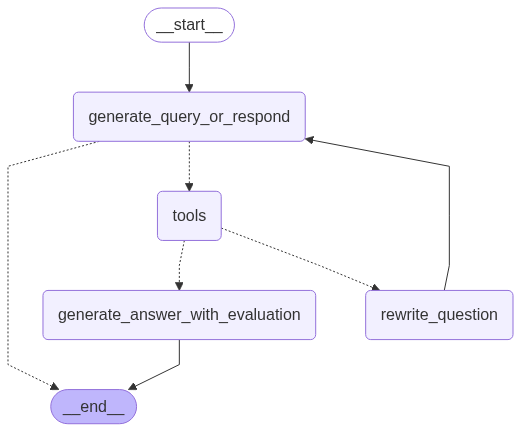
\includegraphics[width=0.8\textwidth]{langgraph_workflow.png}
    \caption{Technische uitwerking van de workflow als LangGraph-graaf, waarbij de verschillende nodes de stappen in het proces voorstellen en de pijlen de mogelijke routes aangeven die de LLM kan volgen.}
    \label{fig:langgraph}
\end{figure}

\subsubsection{Antwoorden of documenten ophalen}

Vooraleer het RAG-proces op gang wordt gebracht, moet de LLM eerst een inschatting maken over de vraag die de gebruiker heeft gesteld. Wanneer het gaat om een triviale vraag, dient de LLM onmiddellijk een antwoord te geven, zonder het volledige RAG-proces te doorlopen. Om dit te realiseren, wordt gebruikgemaakt van de volgende prompt, waarin de input van de gebruiker wordt geïnjecteerd: 

\begin{lstlisting}[basicstyle=\small, frame=single, breaklines=true, postbreak=\mbox{\textcolor{red}{$\hookrightarrow$}\space}, escapeinside ={\%,}, escapechar={!}, numbers=left, language=Python, caption=Prompt voor beslissen tussen direct antwoord of documentopvraging]
RETRIEVE_DOCUMENTS_OR_RESPOND_PROMPT = """
    This method decides whether to call the retriever tool or respond directly.
    
    If the user's question is trivial, respond directly. Just respond directly. Do not show your reasoning or thinking process.
    If the question is non-trivial, use the retriever tool to generate a response.
    If in doubt, use the retriever tool to make sure.
    
    Given the user's question:  
    "{message}"
    
    Determine whether the question is trivial. 
"""
\end{lstlisting}

Het voordeel van deze aanpak is dat geen onnodige resources worden verbruikt bij het uitvoeren van het RAG-proces. Enkel wanneer de vraag van de gebruiker effectief nood heeft aan specifieke contextuele informatie, wordt de retriever geactiveerd.
\\[1em]
De LLM krijgt een retriever tool ter beschikking en kan vervolgens autonoom beslissen of deze tool wordt gebruikt of dat er meteen een antwoord gegenereerd wordt. Dit wordt geïmplementeerd in de volgende functie:

\begin{lstlisting}[basicstyle=\small, frame=single, breaklines=true, postbreak=\mbox{\textcolor{red}{$\hookrightarrow$}\space}, escapeinside ={\%,}, escapechar={!}, numbers=left, language=Python, caption=Functie die beslist tussen direct antwoord en documentopvraging]
def retrieve_documents_or_respond(state: MessagesState) -> MessagesState:
    """
    This methods will call the retriever tool when given a non trivial question is asked.
    In the case of a trivial question it will simply provide a response
    Call the model to generate a response based on the current state. Given
    the question, it will decide to retrieve using the retriever tool, or simply respond to the user.
    """
    message = state["messages"][-1].content
    
    prompt = RETRIEVE_DOCUMENTS_OR_RESPOND_PROMPT.format(message=message)
    
    response_model_with_tools = response_model.bind_tools([myminfin_retriever_tool])
    response = response_model_with_tools.invoke([SystemMessage(content=prompt),
    HumanMessage(content=message)])
    return MessagesState(messages=[response])
\end{lstlisting}

In deze stap ontvangt de LLM twee afzonderlijke berichttypes, een SystemMessage en een HumanMessage. De SystemMessage bevat instructies voor het model hoe het dient te handelen. De oorspronkelijke gebruikersvraag wordt hierbij in de prompt \verb|(RETRIEVE_DOCUMENTS_OR_RESPOND_PROMPT)| geïntegreerd, zodat de LLM beschikt over context en richtlijnen voor de verdere verwerking.
\\[1em]
Daarnaast wordt de gebruikersvraag ook afzonderlijk toegevoegd als een HumanMessage. Dit berichttype geeft expliciet aan dat de inhoud afkomstig is van een menselijke gebruiker.
\\[1em]
Tijdens de implementatie is gebleken dat het opnemen van beide berichttypes noodzakelijk is om optimale resultaten te behalen. De SystemMessage verschaft duidelijke instructies en context, terwijl de HumanMessage de oorspronkelijke vraag onvervormd aan het model doorgeeft. Op deze manier beschikt het model zowel over specifieke richtlijnen en het exacte bericht van de gebruiker, wat de kans op correcte interpretatie en verwerking vergroot.

\subsubsection{Retriever}

Zodra de keuze wordt gemaakt om documenten op te halen, spreekt het model de retriever-tool aan. Deze tool raadpleegt ChromaDB om, op basis van een vooraf bepaalde retrieval methode, de relevante documenten op te halen. Er zijn verschillende methoden beschikbaar om chunks uit de vectordatabank op te vragen. Na het testen van meerdere opties werd gekozen voor de \verb|similarity search| methode.
\\[1em]
De alternatieve ophaalmethoden bleken minder geschikt tijdens het testen. Het eerste alternatief, \verb|similarity_score_threshold|, vertoont overeenkomsten met de gebruikte \verb|similarity search|, in de zin dat eveneens de meest relevante documenten worden opgehaald. Het verschil is dat bij deze aanpak een vooraf ingestelde relevantie drempelwaarde vereist is. Alleen chunks die voldoen aan deze drempel worden uit de vectordatabase opgehaald. In de praktijk leidde dit ertoe dat bij bepaalde vragen geen enkele chunk als relevant werd beschouwd, waardoor de vraag niet kon worden beantwoord. Dit ondanks het feit het antwoord wel aanwezig was in de vectordatabase.  
\\[1em]
Het tweede alternatief, \textit{Maximal Marginal Relevance} (MMR), kiest daarentegen bewust voor zo veel mogelijk variatie in de opgehaalde chunks. Dit resulteerde echter vaak in documenten die onvoldoende relevant waren ten opzichte van de gestelde vraag.  
\\[1em]
Om die redenen werd uiteindelijk gekozen voor de \verb|similarity search| methode. Deze functie selecteert de documenten die het meest relevant zijn voor de vraag. In deze PoC specifiek worden bij elke bevraging de vier meest relevante documenten uit de vectordatabase opgehaald.

\subsubsection{Beoordeling documenten}

Na het ophalen van de documenten moet de LLM opnieuw evalueren of het over voldoende informatie beschikt om een antwoord te formuleren. Indien de documenten voldoende relevantie vertonen ten opzichte van de oorspronkelijke vraag, wordt overgegaan tot het genereren van een antwoord. Indien dit niet het geval is, zal de oorspronkelijke vraag geherformuleerd worden en wordt het ophaal proces opnieuw opgestart.

\begin{lstlisting}[basicstyle=\small, frame=single, breaklines=true, postbreak=\mbox{\textcolor{red}{$\hookrightarrow$}\space}, escapeinside ={\%,}, escapechar={!}, numbers=left, language=Python, caption=Functie die beslist tussen antwoord genereren of vraag herschrijven]
def grade_documents(
state: MessagesState,
) -> Literal["generate_answer", "rewrite_question"]:
    """Determine whether the retrieved documents are relevant to the question."""
    
    # Shortcut: If too many messages (multiple rewrites), stop rewriting
    if len(state["messages"]) >= 5:
    return "generate_answer"
    
    question = state["messages"][0].content
    context = state["messages"][-1].content
    
    prompt = GRADE_DOCUMENTS_PROMPT.format(question=question, context=context)
    response = (
    grader_model
        .with_structured_output(GradeDocuments)
        .invoke([HumanMessage(content=prompt)])
    )
    score = response.binary_score
    
    if score == "yes":
        return "generate_answer"
    else:
        return "rewrite_question"
\end{lstlisting}

Om te vermijden dat de LLM de initiële vraag eindeloos blijft herformuleren, wordt gecontroleerd hoe lang de array van de MessagesState is. Wanneer het aantal berichten gelijk is aan of groter is dan 5 (wat neerkomt op maximaal twee herformuleringen), wordt het model verplicht om door te gaan naar de node die verantwoordelijk is voor het genereren van een antwoord. Op die manier wordt gegarandeerd dat de gebruiker een antwoord ontvangt en de LLM niet in een oneindige lus terecht komt.
\\[1em]
Om ervoor te zorgen dat de LLM deze vraag op een correcte manier gaat verwerken worden zowel de opgehaalde documenten als de originele vraag in een prompt toegevoegd. Hierna is het aan de LLM om een oordeel te vellen over de opgehaalde documenten en de mate waarin deze relevant en nuttig zijn om de vraag te beantwoorden.
\begin{lstlisting}[basicstyle=\small, frame=single, breaklines=true, postbreak=\mbox{\textcolor{red}{$\hookrightarrow$}\space}, escapeinside ={\%,}, escapechar={!}, numbers=left, language=Python, caption=Prompt om opgehaalde documenten te beoordelen op basis van de gestelde vraag]
GRADE_DOCUMENTS_PROMPT = (
    "You are a grader assessing relevance of a retrieved document to a user question. \n "
    "Here are the retrieved documents: \n\n {context} \n\n"
    "Here is the user question: {question} \n"
    "If the document contains keyword(s) or semantic meaning related to the user question, grade it as relevant. \n"
    "Give a binary score 'yes' or 'no' score to indicate whether the document is relevant to the question."
)
\end{lstlisting}

\subsubsection{Genereren antwoord}

Wanneer het hele proces doorlopen is moet de LLM aan de slag met de opgehaalde documenten en de vraag van de gebruiker. Het is hierbij de bedoeling dat het antwoord geformuleerd wordt in de taal waarin ze origineel werd gesteld. Ook wanneer de LLM de vraag heeft herschreven en geherformuleerd heeft in een andere taal. Om hallucinaties te voorkomen, wordt expliciet gevraagd om alleen een antwoord te geven wanneer de informatie beschikbaar is in de context. Indien dit niet het geval is, moet de LLM dit ook aan de gebruiker melden. Daarnaast wordt gevraagd om bronnen te vermelden indien mogelijk. Hiervoor werd de volgende prompt gebruikt: 

\begin{lstlisting}[basicstyle=\small, frame=single, breaklines=true, postbreak=\mbox{\textcolor{red}{$\hookrightarrow$}\space}, escapeinside ={\%,}, escapechar={!}, numbers=left, language=Python, caption=Prompt voor genereren van antwoord op basis van de opgehaalde context]
GENERATE_ANSWER_PROMPT = (
    "You are a helpful assistant supporting users with their MyMinfin IT-related questions.\n"
    "Based on the following context, please provide a clear and complete answer.\n"
    "If the answer is not available in the context, kindly let the user know that you don't have enough information.\n"
    "If the context contains a source, always mention it in your answer as the reference.\n"
    "Always respond in the same language this question {question} is asked, even if the context is in a different language.\n"
    "Do not use Markdown or any special formatting in your answer, respond in plain text only.\n\n"
    "Question: {question}\n"
    "Context: {context}"
)
\end{lstlisting}

\subsection{LLM-model}

Nu een duidelijk beeld is geschetst van de structuur van de graaf, kan worden bekeken welke modellen in aanmerking komen voor gebruik. Hierbij gelden enkele beperkingen. Ten eerste wordt gebruikgemaakt van zogenoemde open modellen. Een tweede, hieraan gerelateerde beperking, zijn de hardwarebeperkingen waarmee deze PoC wordt uitgevoerd. Omdat de modellen lokaal draaien, is het niet mogelijk modellen te gebruiken die meer RAM vereisen dan wat op de lokale hardware beschikbaar is. Concreet betekent dit dat alleen modellen met maximaal acht miljard parameters in aanmerking komen. Tot slot moeten de modellen in staat zijn tool calls uit te voeren. Op basis van deze criteria en rekening houdend met de rangschikking op Hugging Face, is de volgende lijst van mogelijke modellen opgesteld:

\begin{itemize}
    \item llama-3.1-8b-instruct
    \item llama-3.2
    \item Mistral-7b-instruct
    \item Qwen2.5-7B instruct
    \item smollm2-1.7b-instruct
    \item granite-3.2-8b-instruct
    \item granite-3.3
    \item Qwen3
\end{itemize}

Tijdens het testen van de PoC werden echter enkele problemen vastgesteld met de tool calls. Dit leidde ertoe dat een aantal modellen niet langer gebruikt kon worden. Dit wordt verder toegelicht in subsectie \ref{tool-calls}.

\begin{itemize}
    \item Mistral-7b-instruct
    \item smollm2-1.7b-instruct
    \item granite-3.2-8b-instruct
    \item granite-3.3
\end{itemize}

Aangezien de bovenstaande modellen niet langer bruikbaar bleken, is ervoor gekozen om voor de PoC en de vergelijkende studie de volgende modellen te gebruiken:

\begin{itemize}
    \item llama-3.1-8b-instruct
    \item llama-3.2
    \item Qwen2.5-7B instruct
    \item Qwen3
\end{itemize}


\section{Problemen en oplossingen}

Tijdens de ontwikkeling van de toepassing deden zich verschillende problemen voor. Zo waren er uitdagingen bij het efficiënt parsen van documenten, het uitvoeren van tool calls en het onverwachte gedrag van de LLM bij het werken met een graafstructuur. Voor elk van deze problemen werd een passende oplossing gezocht en geïmplementeerd.

%Waar liep je tegenaan tijdens de implementatie?
\subsection{Document parsing}
Het parsen van documenten naar embeddings bleek een uitdagend proces. Initieel werd gewerkt met PDF-bestanden maar deze leverden niet altijd het gewenste resultaat op. Dezelfde problemen traden eveneens op bij Word-documenten. De moeilijkheden deden zich vooral voor bij documenten met ongestructureerde elementen. Bij documenten met tabellen ging de structuur na het parsen vaak verloren.
\\[1em]
Een goede parsing is echter cruciaal voor een goed functionerende RAG-oplossing. Wanneer documenten niet correct gestructureerd zijn, kan dit problemen veroorzaken. Worden deze documenten vervolgens als embeddings opgeslagen in de vectordatabase, dan kan de gebrekkige structuur opnieuw in de context terechtkomen die de LLM gebruikt. Dit kan leiden tot problemen bij het genereren van kwalitatieve antwoorden.
\\[1em]
Om dit probleem te verhelpen, werden de documenten in een eerste fase omgezet naar docx-bestanden. Aangezien dit eveneens niet het gewenste resultaat opleverde, werd uiteindelijk gekozen om de documenten te converteren naar Markdown formaat. Deze aanpak had als voordeel dat de documentstructuur tijdens het parsen beter behouden bleef. Dit resulteerde in beter gestructureerde, relevante chunks die vervolgens als context konden worden gebruikt bij het beantwoorden van vragen door de LLM. De chunks in PDF, docx en Markdown kunnen worden geconsulteerd in bijlage \ref{chunks-verschillende-formaten}

\subsection{Tool calls}
\label{tool-calls}

Omdat in de graaf gebruik wordt gemaakt van een tool, is het noodzakelijk om modellen te gebruiken die in staat zijn om tool calls uit te voeren. Hierdoor is het in deze PoC bijvoorbeeld niet mogelijk om met Google's Gemma modellen te werken, aangezien deze modellen geen ondersteuning bieden voor tool calls.
\\[1em]
Hoewel sommige Ollama modellen wel tool calls ondersteunen, blijkt uit de praktijk dat deze functionaliteit niet altijd betrouwbaar is. Ondanks dat de modellen technisch gezien tool calls kunnen uitvoeren, levert dit niet altijd het gewenste resultaat op.
\\[1em]
Bij het bepalen van de modellen voor de vergelijkende studie werd dan ook vastgesteld dat testen met een aantal modellen onmogelijk was, omdat de vereiste tool call naar de retriever simpelweg niet werd gegenereerd. 

\begin{figure}[H]
    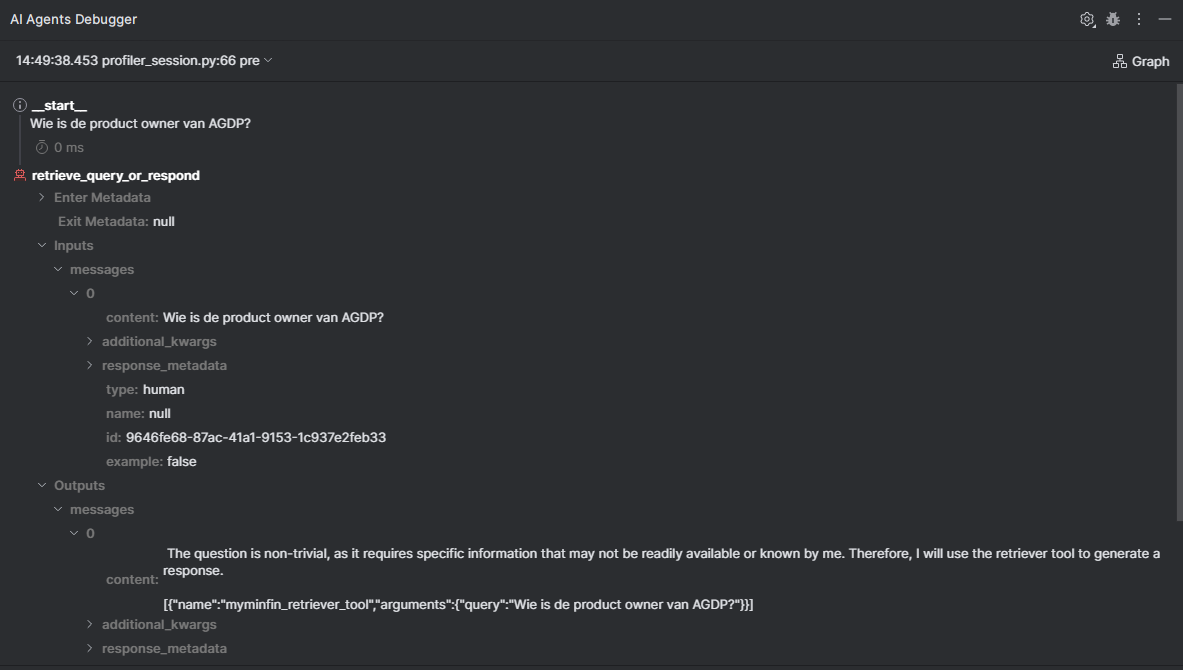
\includegraphics[width=0.8\textwidth]{mistral.png}
    \caption{Tool call bij het Mistral:7b model}
    \label{fig:Mistral}
\end{figure}

De figuur~\ref{fig:Mistral} illustreert waar het fout loopt bij dit model. Ondanks dat het model zich bewust is van de aanwezigheid van de tool en correct inschat dat de gestelde vraag niet triviaal is, wordt de tool call toch niet effectief uitgevoerd.
\\[1em]
Opmerkelijk is dat de tool call met de juiste parameters wel aanwezig is in de content van het antwoord, maar deze wordt niet als daadwerkelijke tool call geïnterpreteerd of geactiveerd door het model.
\\[1em]
Dit probleem deed zich voor bij de volgende modellen:
\begin{itemize}
    \item Mistral-7b-instruct
    \item smollm2-1.7b-instruct
    \item granite-3.2-8b-instruct
    \item granite-3.3
\end{itemize}

 Daardoor kunnen deze modellen niet worden gebruikt binnen deze PoC en de bijhorende vergelijkende studie, aangezien ze de vectordatabase nooit aanspreken en dus geen relevante antwoorden aan de gebruiker kunnen bieden.

\subsection{Fout door oneindige herformuleringslus}

Hoewel de LLM in staat is om zelf te bepalen wat een non triviale vraag is, betekent dit niet noodzakelijk dat het antwoord daarop terug te vinden is in de beschikbare documentatie. Zelfs wanneer de informatie wel aanwezig is, kan het alsnog voorkomen dat de LLM, zelfs na herformulering van de vraag, geen passend antwoord weet te genereren. Dit leidde aanvankelijk tot een oneindige lus waarbij uiteindelijk een foutmelding werd gegenereerd zodra de array messages in de MessageState een lengte van 25 bereikte. In dat geval werd er geen antwoord aangemaakt, maar kreeg de gebruiker enkel een foutmelding te zien met stacktrace.
\\[1em]
Om te voorkomen dat het programma in een dergelijke oneindige lus terechtkomt, werd er een extra controle ingebouwd op het moment dat de LLM moet kiezen tussen het herformuleren van de vraag of het genereren van een antwoord. In de praktijk betekent deze controle dat de LLM de vraag maximaal twee keer mag herformuleren. Hierdoor wordt de vectordatabase in totaal maximaal drie keer bevraagd. Indien er na deze pogingen nog steeds geen relevante documenten worden teruggevonden, is het de bedoeling dat de LLM dit expliciet communiceert aan de gebruiker, zonder dat er sprake is van hallucinaties. 

\subsection{Meertaligheid documentatie}
%het gaat hier over het feit dat hij steeds de eerste vraag vertaalde naar het engels.
%Hoe heb je dat opgelost? Eventueel kort uitleggen als dat relevant is.
Bij het testen van de lus ontstond het probleem dat telkens enkel de originele vraag werd herschreven. Hierdoor werd bijvoorbeeld de oorspronkelijke vraag wel correct naar het Engels herschreven, maar bij iedere volgende iteratie werd opnieuw exact dezelfde vertaling gegenereerd. Er werd met vorige pogingen geen rekening gehouden.
\\[1em]
Om dit probleem op te lossen, werd de prompt in de \verb|rewrite_question| node aangepast zodat de LLM ook rekening kan houden met de eerder gestelde en herschreven vragen. Dit voorkomt herhaling en zorgt voor meer variatie in de gegenereerde vragen.
\\[1em]
Aangezien het grootste deel van de beschikbare documentatie in het Frans of Engels is geschreven, wordt de LLM eveneens aangemoedigd om de vraag eerst naar het Frans te herschrijven en vervolgens, indien nodig, naar het Engels.

\begin{lstlisting}[basicstyle=\small, frame=single, breaklines=true, postbreak=\mbox{\textcolor{red}{$\hookrightarrow$}\space}, escapeinside ={\%,}, escapechar={!}, numbers=left, language=Python, caption=Prompt om vraag te herschrijven]
REWRITE_QUESTION_PROMPT = (
    "You are assisting with improving a user's question related to Myminfin IT support.\n"
    "Conversation history so far (most recent last):"
    "\n ------- \n"
    "{questions}"
    "\n ------- \n"
    "Original question:"
    "\n ------- \n"
    "{original_question}"
    "\n ------- \n"
    "Rewrite the last question to make it short, clear, and easy to match with relevant documents in a vector database.\n"
    "- Keep the meaning and intent exactly the same.\n"
    "- Use simple, direct wording without adding unnecessary details.\n"
    "- If the question is in Dutch, rewrite and translate it to French.\n"
    "- If the question is in French, rewrite and translate it to English.\n"
    "- Avoid repeating previous questions word-for-word.\n"
    "- If it’s similar to a previous question, add only minimal context needed for distinction.\n"
    "- Return only the rewritten question."
)
\end{lstlisting}
\section{Samenvatting}

%Korte recap: wat is gebouwd en werkt zoals verwacht?
%Eventueel: wat is nog niet geïmplementeerd en waarom niet (scope, tijdsbeperkingen)?

Het eindresultaat van deze PoC is een chatinterface die kan worden gebruikt om gerichte vragen te stellen aan de IT-support voor MyMinfin. De toepassing werkt zoals verwacht: afhankelijk van de vraag worden relevante documenten opgehaald en wordt de nodige informatie aan de eindgebruiker verstrekt. Hoewel de hoeveelheid documentatie nog verder opgeschaald kan worden, vormt dit een sterke eerste stap in het opzetten van een ondersteunende tool voor de dagelijkse supportwerking.
\\[1em]
Toch zijn er ook enkele zaken die momenteel nog ontbreken. Zo zou het nuttig zijn indien de agent zelfstandig documentatie kan aanpassen of aanvullen. Dit zou ervoor zorgen dat de beschikbare informatie steeds up-to-date blijft, zonder dat hiervoor handmatige tussenkomst van gebruikers nodig is. Deze functionaliteit viel echter buiten de scope van deze PoC en kon, omwille van tijdsbeperkingen, niet worden gerealiseerd.
\\[1em]
Daarnaast beschikt de huidige LLM-toepassing niet over enige vorm van geheugen. Bij elke nieuwe vraag begint de LLM volledig van nul, zonder kennis van eerdere interacties binnen dezelfde sessie. Er is dus geen sprake van contextopbouw of het onthouden van vorige vragen en antwoorden, wat de gebruikservaring momenteel beperkt tot losstaande interacties.